\documentclass[a4paper,oneside,11pt]{memoir}

\usepackage[utf8]{inputenc} % input encoding
\usepackage[T1]{fontenc} % font encoding

\usepackage{graphicx} %to include images/graphics
\usepackage{amsmath,amssymb} %better math type setting
\usepackage{listings} %for source code snippets
\usepackage{textcomp} %for upquote
\usepackage{xcolor} % nice colors (for source code)
\usepackage{microtype} % subtle font expansion/protrusion to reduce overfull boxes
\usepackage{xurl} % allow long URLs (bibliography) to break instead of overflowing
\usepackage{tikz} % component diagram and other vector graphics
\usetikzlibrary{positioning,arrows.meta,shapes.geometric,fit,backgrounds,calc}

% Listing style for AI prompts shown in the Declaration of AI usage.
\lstdefinestyle{prompt}{
        basicstyle=\ttfamily\footnotesize,
        frame=single,
        backgroundcolor=\color{black!3},
        breaklines=true,
        breakatwhitespace=true,
        breakindent=1em,
        columns=fullflexible,
        keepspaces=true,
        xleftmargin=1em,
        xrightmargin=1em,
}

\renewcommand{\ttdefault}{pcr} % nicer font for source code

% Allow LaTeX more slack when breaking paragraphs to avoid overfull lines.
\setlength{\emergencystretch}{3em}
\tolerance=2000

% Discretionary break helper: inserts an allowed line-break point.
% Use inside long inline literals, e.g. \texttt{--hyperband\bk\_initial\bk\_children}
\newcommand{\bk}{\discretionary{}{}{}}

% Enable hyphenation inside \texttt{}: long identifiers like
% --hyperband_initial_children can then break across lines.
\makeatletter
\DeclareRobustCommand\ttfamily
        {\not@math@alphabet\ttfamily\mathtt
         \fontfamily\ttdefault\selectfont
         \hyphenchar\font=`\-\relax}
\makeatother

% an example configuration of the 'listings' package
\lstset{basicstyle=\ttfamily\small,
        keywordstyle=\color{purple}\ttfamily,
        commentstyle=\color{gray}\ttfamily,
        stringstyle=\color{orange}\ttfamily,
        captionpos=b,
        float=tb,
        upquote=true,
        breaklines=true,
        breakatwhitespace=true,
        breakindent=2em,
        columns=fullflexible,
        postbreak=\mbox{\textcolor{gray}{$\hookrightarrow$}\space},
}

\chapterstyle{tandh} % configuration of the 'memoir' class

%
% The actual document starts here
%
\begin{document}

\begin{titlingpage}
\thispagestyle{empty}

\centering
  \vspace*{6.5em}

  \textsc{\textbf{\huge
      A Comparative Study of Multi-Fidelity \\[\onelineskip]
      Schedulers for Self-Improving \\[\onelineskip]
      Coding Agents
  }}

  \vspace{4.5em}

  \textsc{\Large
    \setlength{\tabcolsep}{12pt}
    \begin{tabular}[h]{lr}
      Leonardo Gianola         &  % TODO: exam number
      \\[.4\onelineskip]
    \end{tabular}
  }

  \vspace{5em}
  \large
  Bachelor Project in Software Engineering

  \normalsize
  \vspace{2em}
  May 2026


  \vspace{12.5em}
  
\includegraphics[width=.5\textwidth]{sdu_logo}

  \vspace{3em}
  The Maersk Mc-Kinney Moeller Institute

  \medskip
  University of Southern Denmark

\end{titlingpage}


\cleardoublepage

\frontmatter

% abstract / resume
\begin{abstract}
  The Darwin G{\"o}del Machine (DGM) is an evolutionary framework in which a
  population of coding agents repeatedly self-modifies, evaluates the resulting
  children on a software engineering benchmark, and keeps the most promising
  variants in an archive.  Each generation spends most of its compute budget on
  evaluating children that ultimately fail to improve the parent.  This thesis
  investigates whether \emph{multi-fidelity evaluation schedulers} can reduce
  wasted compute without sacrificing the final accuracy of the evolved agents.

  We extend the DGM with four schedulers --- a sequential \texttt{baseline},
  synchronous \texttt{hyperband}, asynchronous \texttt{asha}, and a blind
  high-temperature genetic algorithm \texttt{ga} --- and compare them on a
  fixed subset of SWE-bench Verified (\texttt{swe\_verified\_mini}, 50 tasks)
  using the same self-improvement budget, model, and initial archive.
  % TODO: state main results once experiments complete
\end{abstract}


\cleardoublepage

% Declaration of generative AI usage
\section*{Declaration of generative AI and AI-assisted technologies}
During the preparation of this work the author used generative AI
services and tools in order to find resources, research relevant topics,
review prose, and generate code. After using these tools, the author
reviewed and edited the content as needed and takes full responsibility
for the content of this project. In compliance with the code of conduct
for the use of AI at SDU \cite{SDU-AI-CoC}.

\subsection*{Source and literature search}
Claude Code \cite{claude-code} configured with the Claude Opus 4.6 and
Opus 4.7 models \cite{claude-opus} was used as an interactive assistant
to surface candidate references and to cross-check citations against
their sources. An example prompt used during this process looks like
the following:

\begin{lstlisting}[style=prompt]
I am writing the Background chapter of a bachelor thesis on multi-fidelity schedulers (Successive Halving, Hyperband, ASHA) applied to a self-improving coding agent. Can you list the canonical references for each of these methods and verify whether the Karnin et al. 2013 paper is the correct primary citation for Successive Halving?
\end{lstlisting}

\subsection*{Brainstorming and idea generation}
Claude Code \cite{claude-code} was used to discuss design alternatives
for the scheduler implementations and the experimental protocol. Two
recurring use-cases:
\begin{enumerate}
    \item Scheduler design discussions: clarifying the difference
    between synchronous Hyperband and ASHA, sanity-checking the
    promotion-quota formulation, and reviewing the per-rung budget
    accounting. An example prompt used in this stage:
    \begin{lstlisting}[style=prompt]
In ASHA, the promotion quota per rung is computed as max(1, ceil(n / eta^(r+1))). Is this a cumulative cap on total promotions ever from rung r, or a per-rung count refreshed each time a candidate finishes? I want to make sure my implementation matches the original Li et al. 2020 paper.
    \end{lstlisting}
    \item Experimental-protocol brainstorming: identifying threats to
    validity, choosing diagnostic metrics, and deciding which
    constants to fix across runs. An example prompt used in this
    stage:
    \begin{lstlisting}[style=prompt]
I am running one seed per scheduler on swe_verified_mini, four generations each, fixed initial archive. What are the main threats to validity I should disclose, and which diagnostic metrics would help a reader judge whether the cost-vs-accuracy comparison is fair?
    \end{lstlisting}
\end{enumerate}

\subsection*{Programming}
Agentic coding was used during the implementation phase of the project
for editing the fork of the Darwin G\"odel Machine repository, in
particular the scheduler layer and the operational guards described in
Chapter~\ref{chap:implementation}. For this purpose, the tool below has
been used:
\begin{itemize}
    \item Claude Code \cite{claude-code} with the Claude Opus 4.6 and
    Opus 4.7 models \cite{claude-opus} - the only configuration used
    in the project, for planning, implementing, reviewing diffs,
    locating code across the fork, and assisting with debugging of
    Docker, OpenRouter, and SWE-bench harness integration issues.
\end{itemize}
All AI-generated code was reviewed, tested, and integrated by the
author; the author takes full responsibility for the final
implementation.

\subsection*{Language proofreading or linguistic feedback}
Claude Code \cite{claude-code} was used to review and iterate on the
prose of the thesis. The author wrote the chapter body text by hand;
the model was used to flag unclear sentences, inconsistent terminology,
and structural issues in already-written passages, and to suggest
rewordings that the author then accepted, rejected, or rewrote. The
model was not used to ghostwrite chapter body text. An example prompt
used in this stage:

\begin{lstlisting}[style=prompt]
Review this paragraph for clarity and internal consistency with the rest of the Method chapter. Flag any sentence whose meaning is ambiguous, any term used inconsistently with earlier sections, and any claim that is stronger than what the single-seed pilot data supports. Do not rewrite the paragraph; list the issues.
\end{lstlisting}


\cleardoublepage

\tableofcontents

\mainmatter

%
% We have one file per chapter:
%

% Introduction chapter in 'chap-introduction.tex'
\chapter{Introduction}
\label{chap:introduction}

Large language models (LLMs) have become competent enough at routine
programming tasks that they are now packaged as autonomous \emph{coding
agents}: programs that read a task description, browse a code base, edit
files, run tests, and iterate until the task is solved.  The Darwin
G{\"o}del Machine (DGM)~\cite{Sakana:25} pushes this idea one step further by
letting a coding agent \emph{rewrite its own implementation}.  At every
generation a population of agents proposes modifications to its own source
code, the modified agents are evaluated on a software engineering benchmark,
and the most promising variants are kept in an archive that seeds the next
generation.

\section{Problem}

DGM's evaluation step dominates the wall-clock cost of a run.  Each candidate
child is executed against a benchmark of real GitHub issues, which is both
slow (minutes per task) and monetarily expensive (LLM API calls plus
container time).  Most generated children either fail to compile, regress
relative to the parent, or change behaviour in ways that are only obvious on
a subset of the benchmark.  Spending the full evaluation budget on every
child is therefore wasteful.

\section{Research Question}

\begin{quote}
  \emph{Can multi-fidelity evaluation schedulers reduce the cost per
  improvement of the Darwin G{\"o}del Machine without lowering the accuracy
  of the evolved agents?}
\end{quote}

To answer this we implement and compare four schedulers --- baseline,
hyperband~\cite{Li:18}, ASHA~\cite{Li:20}, and a blind genetic
algorithm --- on \texttt{swe\_verified\_mini}, a 50-task subset of
SWE-bench Verified~\cite{Jimenez:24}.  All schedulers share the same
self-improvement loop, model
(\texttt{openrouter/minimax/minimax-m2.5}), and initial archive.

\section{Contributions}

\begin{itemize}
  \item An open-source DGM fork with four pluggable schedulers and a
    fair-comparison harness on \texttt{swe\_verified\_mini}.
  \item A compile-time argparse guard that rejects self-modifications which
    remove flags required by the evaluation driver, preventing silent budget
    burn on broken children.
  \item % TODO: empirical contribution sentence after Phase 1--3 finish
\end{itemize}

\section{Outline}

Chapter~\ref{chap:background} reviews the DGM, multi-fidelity scheduling, and
SWE-bench.  Chapter~\ref{chap:analysis-and-design} describes the experimental
design and scheduler variants.  Chapter~\ref{chap:implementation} details the
DGM fork, scheduler implementations, and operational guards.
Chapter~\ref{chap:results} reports the empirical comparison.
Chapter~\ref{chap:conclusion} discusses limitations and future work.


% Background chapter in 'chap-background.tex'
\chapter{Background}
\label{chap:background}

This chapter introduces the three building blocks the thesis combines: the
Darwin G{\"o}del Machine (Section~\ref{sec:dgm}), multi-fidelity evaluation
schedulers (Section~\ref{sec:multifidelity}), and the SWE-bench evaluation
suite (Section~\ref{sec:swebench}).

\section{The Darwin G{\"o}del Machine}
\label{sec:dgm}

The Darwin G{\"o}del Machine~\cite{Sakana:25} is an evolutionary
self-improvement loop over coding agents.  An \emph{agent} is a directory
containing the Python source of an LLM-driven program that, given a problem
statement and a Git repository, attempts to produce a patch that solves the
problem.  Each generation proceeds in three phases:
%
\begin{enumerate}
  \item \textbf{Parent selection.}  A scoring rule picks parents from the
    archive of previously-kept agents.
  \item \textbf{Child generation.}  Each parent is asked to propose a
    modification to its own source code; the modified code becomes a
    \emph{child}.
  \item \textbf{Child evaluation.}  Each child is run against the benchmark.
    Children that pass quality and compile checks are added to the archive.
\end{enumerate}
%
The archive seeds the next generation, so improvements compound across
generations.

% TODO: cite original DGM paper formally, expand on archive policy and target
% selection (`score_child_prop`, contextlength targeting, etc.)

\section{Multi-Fidelity Evaluation}
\label{sec:multifidelity}

Multi-fidelity methods exploit the observation that cheap, partial
evaluations are often informative enough to discard the worst candidates
before paying for the full evaluation.  Successive halving runs all
candidates at a small budget, keeps the top $1/\eta$ fraction, and re-runs
them at a larger budget; the process repeats until one budget level
remains.  Hyperband~\cite{Li:18} composes successive halving over several
bracket sizes to balance exploration and exploitation.  ASHA~\cite{Li:20} is
an asynchronous variant in which a candidate is promoted to the next rung as
soon as it ranks in the top $1/\eta$ of the candidates that have completed
the current rung, eliminating the synchronous straggler problem.

In this thesis the candidates are children of a DGM generation and the
fidelities are the number of benchmark tasks each child is evaluated on.

\section{SWE-bench and \texttt{swe\_verified\_mini}}
\label{sec:swebench}

SWE-bench~\cite{Jimenez:24} is a benchmark of real GitHub issues from
popular Python projects.  Each task provides a problem statement, a base
commit, and a hidden set of tests that the agent's patch must make pass.
SWE-bench~Verified is a human-validated 500-task subset; we use a 50-task
sub-subset, \texttt{swe\_verified\_mini}, which is small enough to run
multiple full generations within the thesis budget while preserving the
distribution of task difficulties.

% TODO: describe per-task evaluation pipeline (Docker, conda envs, report.py)


% ...

% Analysis and Design chapter in 'chap-analysis-and-design.tex'
\chapter{Method}
\label{chap:analysis-and-design}

This chapter establishes the four scheduler variants and the experimental
protocol used to compare them on the research question: under a fixed
per-generation task budget, which scheduler produces the
highest-performing agent at the lowest cost. All four variants share the
same language model (minimax-m2.5), benchmark, number of generations,
initial archive, seed, and per-generation task budget; differences reside
only in candidate selection and promotion policy, isolating the scheduler
as the sole independent variable. Section~\ref{sec:schedulers} defines
each scheduler and its purpose. Section~\ref{sec:protocol} specifies the
experimental protocol. Section~\ref{sec:metrics} lists the collected
metrics and their relevance to the research question.
Section~\ref{sec:analysis} sets the analysis plan.
Section~\ref{sec:threats} discusses threats to validity.

\section{Subjects Under Comparison}
\label{sec:schedulers}

\paragraph{Baseline.}
Baseline is the base configuration of the system and is used as the
reference scheduler. It evaluates each child through a fixed three-stage
pipeline of cumulative task counts, killing candidates between stages
on a fixed threshold at stage~0 and an archive-relative threshold at
stage~1. The promotion mechanism of this scheduler is based on three
stages: small (3 tasks), medium (12 tasks), and full (35 tasks), for a
total of 50 tasks per fully-evaluated child. To pass from the small to
the medium stage, the child must resolve at least 40\% of the
small-stage tasks. To pass from the medium to the full stage, the
child's cumulative score must meet or exceed the full-evaluation
threshold (the lowest score in the current archive). Once at the full
stage the child is evaluated on the 35 remaining tasks to obtain its
final score.

Shared run controls used by all schedulers:
\texttt{--selfimprove\_size} controls the number of children per
generation; \texttt{--generation\_task\_budget\_total} is the maximum
number of tasks per generation, ensuring a fair budget across schedulers;
\texttt{--selfimprove\_workers} sets the number of evaluations run in
parallel; \texttt{--num\_benchmark\_evals} controls the number of times
each child re-runs the same task subset; \texttt{--benchmark} selects the
benchmark suite (SWE-bench, SWE-bench mini, or polyglot). Other run
controls: seed, max generations, archive update policy, shallow
evaluation, skip-final-evaluation, and evaluation noise.

\paragraph{Hyperband.}
Hyperband is the synchronous Successive Halving implementation for DGM,
where each candidate receives a number of tasks directly proportional to
how well it ranks at each rung. The evaluation is organised into rungs;
each rung evaluates the surviving candidates on its assigned task budget
and keeps the top $1/\eta$ fraction, where $\eta$ is the reduction
factor. $\eta$ controls two things at each rung: the survival fraction
($1/\eta$) and the per-candidate budget growth (approximately
$\eta\times$ larger task budget at the next rung). Per rung: evaluate all
surviving candidates on the incremental tasks, score them by the
cumulative resolution rate across all tasks seen so far, wait for all
evaluations to finish, and promote $\lceil n_r / \eta \rceil$ children
with a positive score. For example, with $n = 15$ and $\eta = 5$:
rung~0 $\rightarrow$ 3 promoted; rung~1 $\rightarrow$ 1 promoted. In the
last rung every surviving candidate is kept.

Hyperband-specific parameters: \texttt{--hyperband\_eta} (the reduction
factor); \texttt{--hyperband\_budgets} (the cumulative task counts at
each rung; default \texttt{2,10,50});
\texttt{--hyperband\_initial\_children} (number of children spawned at
rung~0). This scheduler replaces the baseline's fixed three-stage rule
with a configurable bracket, spending the same task budget on more
candidates and killing the least-promising first.

\paragraph{ASHA.}
ASHA is the asynchronous variant of Hyperband. It uses the same rung
structure and task budgets as Hyperband but never waits for an entire
rung to finish before promoting. The promotion mechanism of ASHA is
conceptually the same as Hyperband but uses a fixed quota per rung
computed at startup: $\max(1, \lceil n / \eta^{r+1} \rceil)$.
Evaluations stream in asynchronously. On each completion at
rung~$r$, ASHA re-ranks all rung-$r$ completions seen so far; if the
candidate has a positive score and currently sits in the top-quota set,
it is promoted to rung~$r+1$ immediately. Otherwise it is dropped and
ASHA continues processing further completions. As soon as a worker slot
frees, the next pending candidate is dispatched, minimising idle time
relative to synchronous Hyperband.

ASHA reuses Hyperband's parameters
(\texttt{--hyperband\bk\_eta}, \texttt{--hyperband\bk\_budgets},
\texttt{--hyperband\bk\_initial\bk\_children}), extending Hyperband
by removing the per-rung synchronisation barrier.

\paragraph{Genetic Algorithm (GA).}
The Genetic Algorithm (GA) scheduler~\cite{Holland:75} is a
blind-evolution control: it preserves DGM's three-stage Baseline
evaluation pipeline but strips error-log context from child
generation. It is used to test whether
DGM's gains come from error-log-guided self-diagnosis or from random
mutations followed by selection. Promotion works exactly the same as
Baseline; the only difference is in child generation, which uses a
high-temperature LLM mutation with no error-log context.

GA-run-specific parameters: \texttt{--ga\_mutation\_temperature}
controls the LLM sampling temperature for blind mutations;
\texttt{--ga\_tournament\_k} controls the tournament
size~\cite{Miller:95} at parent selection (activated by setting
\texttt{--choose\_selfimproves\_method tournament} in
\texttt{DGM\_outer.py}).

\section{Experimental Protocol}
\label{sec:protocol}

The single independent variable across runs is the scheduler choice
(\texttt{--scheduler}), taking one of four values: \texttt{baseline},
\texttt{hyperband}, \texttt{asha}, \texttt{ga}. Four runs were
conducted, one per scheduler.

All other variables are held constant:
\begin{itemize}
  \item \textbf{Language model}: minimax-m2.5 (via OpenRouter).
  \item \textbf{Benchmark}: \texttt{swe\_verified\_mini} (a 50-task
    subset of SWE-bench Verified).
  \item \textbf{Initial archive}: bootstrapped with
    \texttt{test\bk\_swebench.py} on
    \texttt{swe\bk\_verified\bk\_mini} into
    \texttt{initial\bk\_swe\bk\_verified\bk\_mini/}.
  \item \textbf{Random seed}: \texttt{0}.
  \item \textbf{Generations per run}: \texttt{4}
    (\texttt{--max\_generation 4}).
  \item \textbf{Children per generation}: \texttt{2}
    (\texttt{--selfimprove\bk\_size 2}) for Baseline and GA;
    Hyperband and ASHA spawn \texttt{15} instead
    (\texttt{--hyperband\bk\_initial\bk\_children 15}).
  \item \textbf{Per-generation task budget cap}: \texttt{100}
    (\texttt{--generation\bk\_task\bk\_budget\bk\_total 100}).
  \item \textbf{Archive update policy}: \texttt{keep\_all}
    (\texttt{--update\bk\_archive keep\bk\_all}).
  \item \textbf{Benchmark evaluations per child}: \texttt{1}
    (\texttt{--num\_benchmark\_evals 1}).
  \item \textbf{Evaluation noise leeway}: \texttt{0.1}
    (\texttt{--eval\_noise 0.1}).
  \item \textbf{Hardware}: Intel Core i7-12800H (14 cores, 20 threads),
    16~GiB RAM, Fedora Linux 44.
\end{itemize}

A sample run command for Hyperband is given in
Listing~\ref{lst:run-hyperband} (Appendix~\ref{app:reproduction}). The
other three schedulers use identical flags with \texttt{--scheduler}
swapped: see Listings~\ref{lst:run-baseline}, \ref{lst:run-ga},
and~\ref{lst:run-asha} for the Baseline, GA, and ASHA commands. Baseline
drops the three \texttt{--hyperband\_*} flags; GA drops them and adds
\texttt{--ga\_mutation\_temperature 1.0}.

\section{Metrics}
\label{sec:metrics}

The metrics fall into two groups: per-child (recorded in each child's
\texttt{metadata.json}) and per-generation (aggregated and stored in
\texttt{dgm\bk\_metadata.jsonl}). Primary metrics for the research
question are marked \emph{primary}; the rest are \emph{diagnostic}.

\paragraph{Per-child metrics.}
\begin{itemize}
  \item \texttt{accuracy\_score} (\emph{primary}). The rate
    $\mathrm{resolved} / \mathrm{submitted}$ in $[0, 1]$. Empty
    patches count in the denominator (one submitted, zero resolved,
    so they drag the rate down). Tasks with no prediction file at all
    (context-overflow crashes, docker timeouts) drop silently from
    the denominator; see Section~\ref{sec:threats}. Direct measure of
    agent effectiveness on the tasks it actually attempted.
  \item \texttt{is\bk\_compiled} (\emph{diagnostic}). A boolean flag
    (\texttt{is\bk\_compiled\bk\_self\bk\_improve} in
    \texttt{utils/evo\bk\_utils.py}) that is \texttt{True} when the
    child both (a) produced at least one non-empty patch, i.e.\
    $|\mathrm{resolved}| + |\mathrm{unresolved}| > 0$, and (b) has
    \texttt{compile\bk\_failure\bk\_reason} equal to \texttt{None}.
    Tracks wasted budget on children whose patch never compiled or
    was empty.
  \item \texttt{promoted\_from\_rung} (\emph{diagnostic}). Per-child
    integer: the highest rung the child was promoted from
    (\texttt{None} if killed at rung~0). Reveals how aggressively each
    scheduler prunes and how budget is concentrated on survivors.
  \item \texttt{token\bk\_usage\bk\_total} (\emph{primary, cost
    component}). Sum of input + output tokens consumed by the child
    across all LLM calls (mutation generation, evaluation iterations).
    Read directly from
    \texttt{metadata['token\bk\_usage\bk\_total']}. Multiplied by the
    minimax-m2.5 token prices to convert to USD.
  \item \texttt{evaluated\_task\_count} (\emph{diagnostic}). Number of
    distinct tasks the child was actually evaluated on
    (\texttt{total\_submitted\_instances}). Used to determine whether
    the child reached the full budget, and required for inclusion in
    \texttt{best\_child\_score}.
\end{itemize}

\paragraph{Per-generation metrics} (each entry in
\texttt{dgm\_metadata.jsonl}):
\begin{itemize}
  \item \texttt{best\bk\_child\bk\_score} (\emph{primary outcome}).
    $\max(\texttt{accuracy\bk\_score})$ over children whose
    \texttt{evaluated\bk\_task\bk\_count} $\geq$
    \texttt{full\bk\_budget\bk\_size}. Single-number summary of the
    best agent produced in the generation. Tracks DGM's progress over
    generations.
  \item \texttt{children\_fully\_evaluated\_count}
    (\emph{diagnostic}). Number of children whose
    \texttt{evaluated\_task\_count} reached the final rung's task
    budget. Indicates how effective the scheduler was at promoting
    survivors all the way through the pipeline.
  \item \texttt{evaluation\_budget\_tasks\_consumed} (\emph{primary,
    efficiency}). Sum of
    $\mathit{candidates\_at\_rung} \times
    \mathit{tasks\_added\_at\_rung}$
    across all rungs/stages in the generation. The denominator of any
    ``best score per task'' efficiency comparison between schedulers.
  \item \texttt{cost\_per\_gen} (\emph{primary, cost}). Derived (not
    stored):
    $\text{cost} = (\Sigma\ \mathit{input\_tokens}) \times
    \$0.15/\text{M} + (\Sigma\ \mathit{output\_tokens}) \times
    \$1.15/\text{M}$,
    summed across all children in the generation, using
    minimax-m2.5's OpenRouter prices. This is the metric the thesis
    seeks to minimise subject to score gain.
  \item \texttt{generation\_wall\_clock\_seconds}
    (\emph{diagnostic}). Elapsed wall-clock seconds from generation
    start to scheduler return, stored as
    \texttt{generation\_wall\_clock\_seconds}. Captures parallelism
    gains that are invisible to cost and task counts, critical for
    evaluating ASHA's asynchronous claim.
  \item \texttt{archive\_size} and $\Delta$\texttt{archive\_size}
    (\emph{diagnostic}). \texttt{archive\_size} is the cumulative
    count of compiled children in the archive after the generation
    completes; $\Delta$\texttt{archive\_size} is the difference
    between consecutive generations (i.e., the number of new children
    promoted into the archive this generation). Tracks population
    diversity over generations.
\end{itemize}

\section{Analysis Plan}
\label{sec:analysis}

Each scheduler was run once (single seed), so no between-run
aggregation is possible. All analysis is within-run and descriptive,
without significance tests or confidence intervals.

Within each run, the metadata is loaded and the primary metrics
(\texttt{best\bk\_child\bk\_score}, \texttt{cost\bk\_per\bk\_gen},
\texttt{evaluation\bk\_budget\bk\_tasks\bk\_consumed}) are plotted as
a function of generation. Diagnostic metrics
(\texttt{generation\bk\_wall\bk\_clock\bk\_seconds},
\texttt{children\bk\_compiled\bk\_count}, \texttt{archive\bk\_size},
and the \texttt{promoted\bk\_from\bk\_rung} distribution) are plotted
alongside for context. The four schedulers are then compared on the
same axes to
surface differences in trajectory and final state.

The only source of within-run variance is \texttt{--eval\_noise 0.1},
the noise leeway applied to the archive-worst score threshold in
\texttt{update\_archive()}. Score changes below this threshold are not
treated as meaningful improvements.

Aggregated cost, wall-clock, final archive composition, and
best-of-run score per scheduler are reported in
Chapter~\ref{chap:results}, Section~\ref{sec:results-summary}. The best-of-run score is
defined as $\max(\texttt{best\_child\_score})$ across the four
generations of a scheduler's run that is, the best child produced
at any point in the run. Per-generation
trajectories appear in Section~\ref{sec:results-accuracy}. The
cost-vs-score comparison, which is the central result for the research
question, appears in Section~\ref{sec:results-costscore}.

A multi-seed re-run of all four schedulers is required before any
inferential claim can be made; this is deferred to future work.

\section{Threats to Validity}
\label{sec:threats}

Several threats apply to this work.

\paragraph{Internal validity.}
\begin{itemize}
  \item Single-seed-per-scheduler execution: one run per condition, no
    within-scheduler variance estimate, no significance claim possible.
  \item \texttt{accuracy\_score} denominator silently drops tasks for
    which no prediction file was emitted (context-overflow crashes,
    docker timeouts, harness exceptions). Empty patches are counted
    and penalise the rate, but full no-file failures shrink the
    denominator and can inflate the reported rate; minimax-m2.5
    context-overflow crashes on harder tasks expose this bias.
  \item Hyperband and ASHA require score $> 0$ for promotion, killing
    zero-score children regardless of their tie-breaker rank.
  \item \texttt{num\_benchmark\_evals = 1}: each child's score is a
    single-sample estimate of LLM-stochastic performance.
\end{itemize}

\paragraph{External validity.}
\begin{itemize}
  \item Results on the 50-task \texttt{swe\_verified\_mini} subset may
    not generalise to the full SWE-bench Verified (500 tasks), to other
    SWE benchmarks, or to polyglot tasks.
  \item All four runs use minimax-m2.5; scheduler behaviour under
    stronger or weaker LLMs may differ.
  \item Each run is capped at four generations; long-run dynamics are
    not observed.
  \item All four runs start from the same initial archive; biases in
    the seed agent propagate uniformly.
\end{itemize}

\paragraph{Construct validity.}
\begin{itemize}
  \item \texttt{cost\_per\_gen} measures LLM-spend only;
    Docker/infrastructure cost is excluded.
  \item Cost-vs-score framing assumes uniform task value, which
    SWE-bench Verified does not enforce.
  \item Wall-clock comparisons are confounded by background system load
    and OpenRouter latency, particularly relevant for ASHA's
    asynchronous claim.
\end{itemize}


% Implementation chapter in 'chap-implementation.tex'
\chapter{Implementation}
\label{chap:implementation}

This work is an add-on contribution to the Darwin G\"odel Machine paper,
whose code is public.\footnote{\texttt{https://github.com/jennyzzt/dgm.git}}
We forked the repo and added an advanced scheduler mechanism to try to
get as much as possible out of this system. Each scheduler implementation
is in the \texttt{schedulers.py} file. This chapter documents the fork
additions (Section~\ref{sec:fork}), the scheduler implementations
(Section~\ref{sec:scheduler-impl}), and the operational guards that keep
long runs robust (Section~\ref{sec:guards}).

Figure~\ref{fig:components} gives a high-level component view of the
forked system and how the parts interact across a single generation.
The evolution loop in \texttt{DGM\_outer.py} drives a pluggable
scheduler, which delegates child generation and evaluation to
\texttt{self\_improve\_step.py}. Generation flows through the coding
agent and the LLM stack out to the OpenRouter API; evaluation flows
through the benchmark registry and the Docker utilities into a
per-task SWE-bench harness container. Results from both flows are
recorded per child and then appended to \texttt{dgm\_metadata.jsonl},
which feeds the archive consulted by the scheduler in the next
generation.

\begin{figure}[tb]
  \centering
  \resizebox{\textwidth}{!}{%
  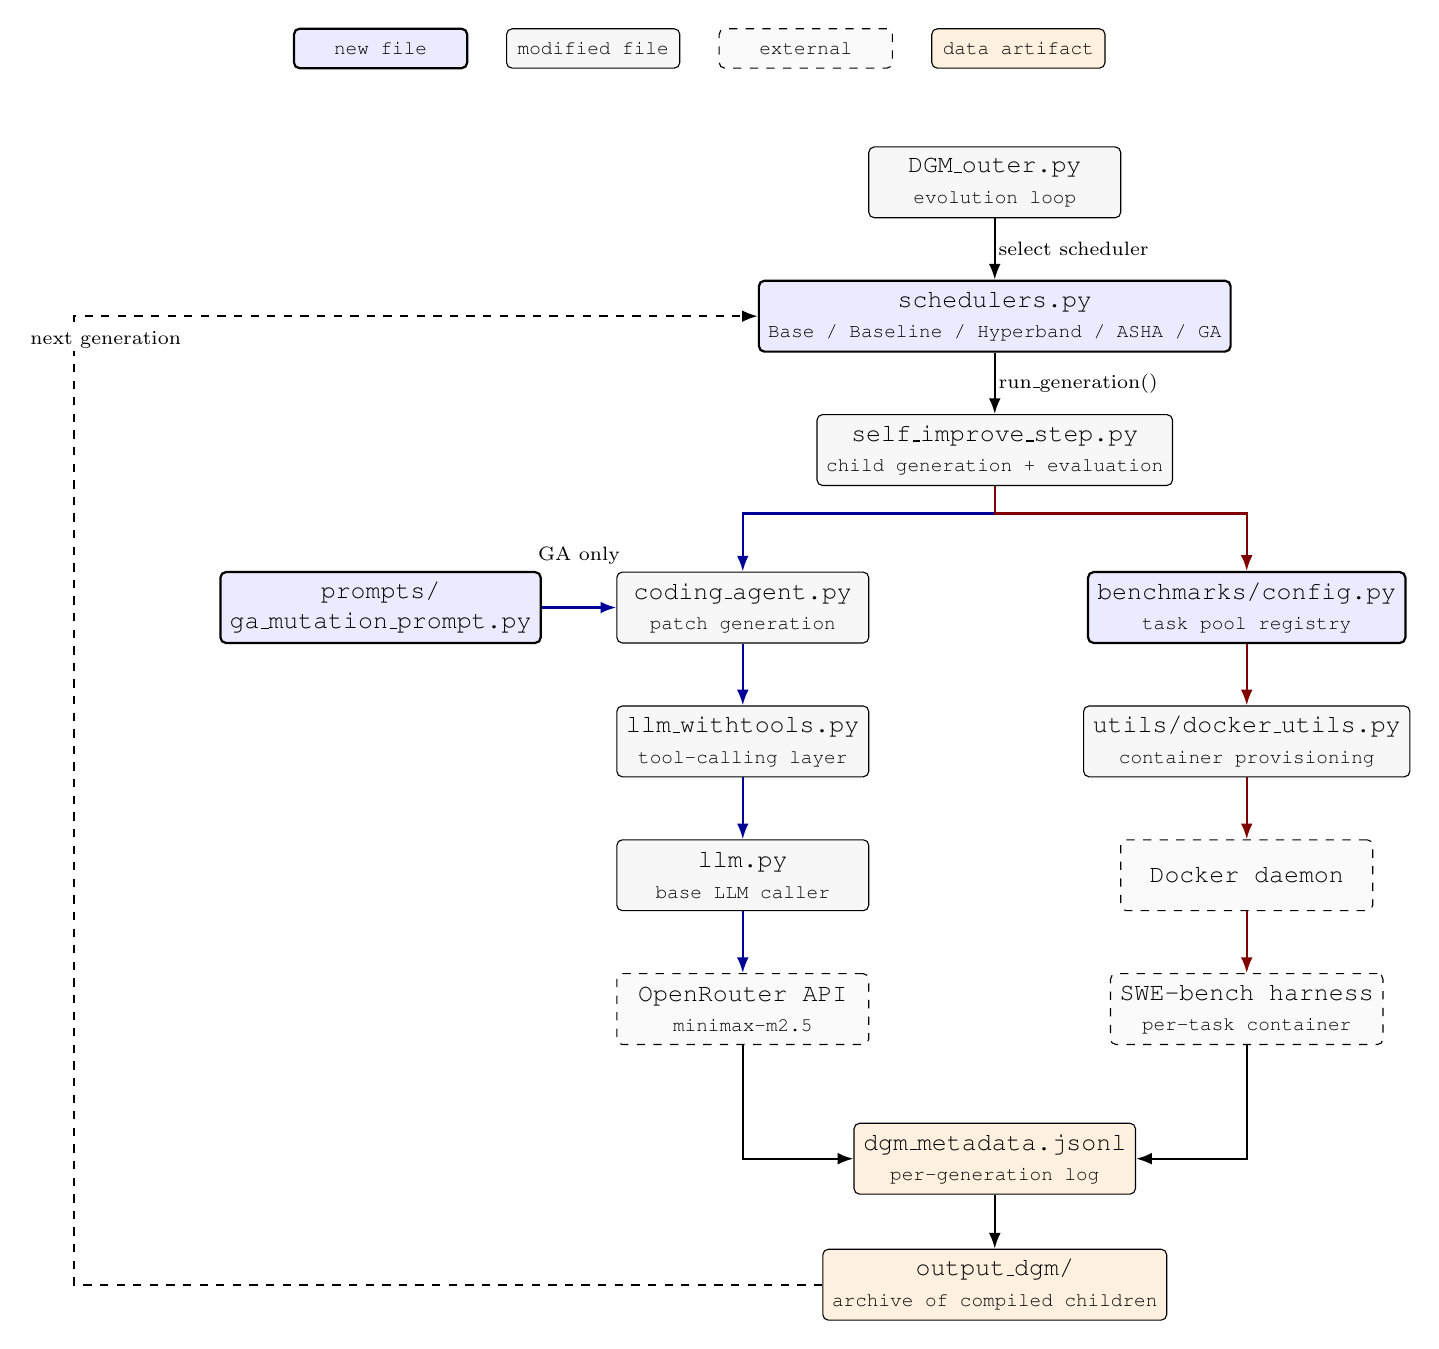
\begin{tikzpicture}[
      font=\small\ttfamily,
      every node/.style={align=center},
      mod/.style={draw, rounded corners=2pt, fill=black!3,
                  minimum width=32mm, minimum height=9mm},
      new/.style={draw, rounded corners=2pt, fill=blue!8,
                  line width=0.8pt,
                  minimum width=32mm, minimum height=9mm},
      ext/.style={draw, dashed, rounded corners=2pt, fill=black!2,
                  minimum width=32mm, minimum height=9mm},
      data/.style={draw, rounded corners=2pt, fill=orange!12,
                   minimum width=32mm, minimum height=9mm},
      flow/.style={-{Latex[length=2mm]}, thick},
      gen/.style={flow, draw=blue!60!black},
      eval/.style={flow, draw=red!50!black},
      lbl/.style={font=\scriptsize\rmfamily, fill=white, inner sep=1pt},
  ]

  % Backbone (centered)
  \node[mod]  (outer)    at ( 0,    0)    {DGM\_outer.py\\\scriptsize evolution loop};
  \node[new]  (sched)    at ( 0,   -1.7)  {schedulers.py\\\scriptsize Base / Baseline / Hyperband / ASHA / GA};
  \node[mod]  (sis)      at ( 0,   -3.4)  {self\_improve\_step.py\\\scriptsize child generation + evaluation};

  % Left column (generation pipeline)
  \node[mod]  (agent)    at (-3.2, -5.4)  {coding\_agent.py\\\scriptsize patch generation};
  \node[new]  (gaprompt) at (-7.8, -5.4)  {prompts/\\ga\_mutation\_prompt.py};
  \node[mod]  (llmwt)    at (-3.2, -7.1)  {llm\_withtools.py\\\scriptsize tool-calling layer};
  \node[mod]  (llm)      at (-3.2, -8.8)  {llm.py\\\scriptsize base LLM caller};
  \node[ext]  (or)       at (-3.2,-10.5)  {OpenRouter API\\\scriptsize minimax-m2.5};

  % Right column (evaluation pipeline)
  \node[new]  (bench)    at ( 3.2, -5.4)  {benchmarks/config.py\\\scriptsize task pool registry};
  \node[mod]  (docker)   at ( 3.2, -7.1)  {utils/docker\_utils.py\\\scriptsize container provisioning};
  \node[ext]  (dock)     at ( 3.2, -8.8)  {Docker daemon};
  \node[ext]  (swe)      at ( 3.2,-10.5)  {SWE-bench harness\\\scriptsize per-task container};

  % Data artifacts (centered, below both columns)
  \node[data] (meta)     at ( 0,   -12.4) {dgm\_metadata.jsonl\\\scriptsize per-generation log};
  \node[data] (archive)  at ( 0,   -14.0) {output\_dgm/\\\scriptsize archive of compiled children};

  % Control flow (backbone)
  \draw[flow] (outer) -- node[lbl, right]{select scheduler} (sched);
  \draw[flow] (sched) -- node[lbl, right]{run\_generation()} (sis);

  % Generation branch
  \draw[gen] (sis.south) -- ++(0,-0.35) -| (agent.north);
  \draw[gen] (agent) -- (llmwt);
  \draw[gen] (llmwt) -- (llm);
  \draw[gen] (llm) -- (or);
  \draw[gen] (gaprompt.east) -- node[lbl, above, yshift=5mm]{GA only} (agent.west);

  % Evaluation branch
  \draw[eval] (sis.south) -- ++(0,-0.35) -| (bench.north);
  \draw[eval] (bench) -- (docker);
  \draw[eval] (docker) -- (dock);
  \draw[eval] (dock) -- (swe);

  % Branch terminals -> metadata (meta sits between or and swe, no archive crossings)
  \draw[flow] (or.south)  |- (meta.west);
  \draw[flow] (swe.south) |- (meta.east);
  \draw[flow] (meta) -- (archive);

  % Feedback arrow routed via far-left margin, well clear of all nodes
  \draw[flow, dashed]
    (archive.west) -- ++(-9.5,0) coordinate (fbk)
    -- (fbk |- sched.west)
    -- (sched.west);
  \node[lbl] at ($(fbk |- sched.west) + (4mm, -3mm)$) {next generation};

  % Legend (top-left, above outer)
  \node[new,  minimum width=22mm, minimum height=5mm, font=\scriptsize\ttfamily] (lg1) at (-7.8, 1.7) {new file};
  \node[mod,  minimum width=22mm, minimum height=5mm, font=\scriptsize\ttfamily] (lg2) at (-5.1, 1.7) {modified file};
  \node[ext,  minimum width=22mm, minimum height=5mm, font=\scriptsize\ttfamily] (lg3) at (-2.4, 1.7) {external};
  \node[data, minimum width=22mm, minimum height=5mm, font=\scriptsize\ttfamily] (lg4) at ( 0.3, 1.7) {data artifact};

  \end{tikzpicture}%
  }
  \caption{Component view of the forked DGM system. Blue-filled boxes
    are files added by this work, grey-filled boxes are files of the
    upstream DGM that were modified, dashed boxes are external
    components (Docker daemon, OpenRouter, SWE-bench harness), and
    orange boxes are persistent data artifacts. Blue arrows trace the
    child-generation pipeline and red arrows trace the evaluation
    pipeline; both converge on \texttt{dgm\_metadata.jsonl}, which
    feeds the archive consulted by the scheduler in the next
    generation.}
  \label{fig:components}
\end{figure}

\section{Fork Additions}
\label{sec:fork}

We forked the Darwin G\"odel Machine repo and modified several files from
the original repo:

\begin{itemize}
  \item \textbf{\texttt{DGM\_outer.py}}: changed the default benchmark to
    SWE-bench Verified Mini; created a scheduler integration with a
    pluggable scheduler hook, re-evaluation-on-promotion budget, new
    metrics, and the ASHA/GA wiring; added the
    \texttt{--generation\_task\_budget\_total} CLI argument
    (\texttt{DGM\_outer.py:277}, default \texttt{None}; the value
    \texttt{100} used in the experiments is a run-time flag, not a code
    default).
  \item \textbf{\texttt{self\_improve\_step.py}}: four big changes. Added
    support for the OpenRouter API key and new models; added the new
    benchmark switch, scheduler budget/metrics, and the GA mutation hook;
    wired the argparse guard. (Note: the Docker repo-copy and container
    git-config fixes are \emph{called} from here but live in
    \texttt{utils/docker\_utils.py}, see Section~\ref{sec:guards}.).
  \item \textbf{\texttt{coding\_agent.py}}: scheduler budget and metrics;
    the empty-patch retry loop (Section~\ref{sec:guards}).
  \item \textbf{\texttt{llm.py}}: the base LLM caller layer. Added the
    model registry entries \texttt{openrouter/minimax/minimax-m2.5} and
    \texttt{openrouter/openai/gpt-5-mini} (\texttt{llm.py:20-21}) as
    usable models, and adapted the layer to keep everything in sync with
    the original code. Minimax is a thinking model, so part of its output
    is a thinking segment wrapped in thinking/JSON tags that must be
    stripped to prevent empty-response failures.
  \item \textbf{\texttt{llm\_withtools.py}}: the tool-calling layer.
    Replaced the default model GPT-5-Mini with Minimax. Created a
    dedicated \texttt{chat.completion} path for Minimax with its standard
    \texttt{tool\_calls} format and no strict mode, because the OpenRouter
    \texttt{chat.completion} schema does not support strict tool-calling.
    It now preserves the full tool-call objects in history, catches
    malformed JSON to skip gracefully without crashing, and mirrors the
    tag-stripping helpers from \texttt{llm.py}.
\end{itemize}

We created new files for the new scheduler mechanisms:

\begin{itemize}
  \item \textbf{\texttt{schedulers.py}}: the entire pluggable scheduler
    layer, containing \texttt{BaseScheduler} plus
    Baseline/Hyperband/ASHA/GA subclasses, per-generation budget
    recording, and timeout constants. This file did not exist in the
    original DGM repo; DGM only had the fixed three-stage evaluation that
    the Baseline scheduler reproduces. This is the core thesis
    contribution: all scheduler logic resides here and the schedulers are
    swappable from one file.
  \item \textbf{\texttt{benchmarks/config.py}}: a configurable test suite
    to select SWE-bench, Polyglot, or SWE-bench Verified Mini. Replaces
    DGM's hardcoded SWE-bench paths. Created because we needed
    reproducible pinned SWE-bench Verified Mini subsets and cumulative
    rung sizes for scheduler evaluation.
  \item \textbf{\texttt{prompts/ga\_mutation\_prompt.py}}: the mutation
    prompt for the genetic algorithm, with no error-log context, asking
    the LLM for random exploration mutations. Reuses the coding-agent
    summary and current-code logic from the self-improvement prompts and
    applies high temperature at call time.
  \item \textbf{\texttt{compare\_scheduler\_runs.py}}: reads all results
    from the \texttt{dgm\_metadata.jsonl} files of the four scheduler runs
    and aggregates them into one JSON for cross-scheduler comparison.
  \item \textbf{\texttt{tests/test\_benchmark\_registry.py}}: verifies the
    pinned, cumulative benchmark subset and keeps the legacy benchmarks
    under a legacy register key for backward compatibility. Added because
    a fixed subset size is required for a fair comparison between
    schedulers.
\end{itemize}

\section{Scheduler Implementations}
\label{sec:scheduler-impl}

\subsection{BaseScheduler}

This is the parent scheduler all others override. It defines the contract
abstractly: \texttt{run\_generation(...)} and
\texttt{get\_generation\_child\_count(...)} both
\texttt{raise NotImplementedError}, so subclasses must supply the
implementation. It provides two shared parallel-executor helpers:
\texttt{\_generate\_children(...)} for parallel child-patch generation and
\texttt{\_evaluate\_children(...)} for parallel evaluation. Promotion,
ranking, and metadata-marking are shared module-level helpers
(\texttt{\_promote\_top\_k}, \texttt{\_rank\_children},
\texttt{\_mark\_promotion\_decisions}) that every subclass calls.

The \texttt{BaseScheduler} contract and shared helpers are listed in
Listing~\ref{lst:base-scheduler}
(Appendix~\ref{app:scheduler-pseudocode}).

\subsection{Baseline}

Builds on BaseScheduler and adds five instance attributes: three task-ID
lists \texttt{stage\_small\_issues} / \texttt{stage\_medium\_issues} /
\texttt{final\_stage\_issues} (one per eval stage),
\texttt{expected\_task\_counts} (used to check whether a child ran enough
tasks for its results to be valid), and \texttt{test\_more\_threshold}
(the promotion gate; a child advances if it solves at least this fraction
of the stage). \texttt{get\_generation\_child\_count} returns how many
children to spawn per generation. \texttt{run\_generation} is a linear,
no-loop implementation with three sequential eval blocks; a
\texttt{consumed\_budget} accumulator increments after each block by
number of children $\times$ stage size.

The stage structure is: \textbf{Stage 0 (small)} evaluates all children,
promoting those that resolve at least 40\% of small-stage tasks;
\textbf{Stage 1 (medium)} takes the Stage-0 survivors and promotes those
whose score is greater than or equal to the full-evaluation threshold;
\textbf{Stage 2 (full)} takes the remaining children, evaluates them on the
full suite, and keeps all of them. Every stage promotion has two steps:
(a) a quality gate filtered by the threshold (Stages 0 and 1), then (b) a
budget cap that takes the max number of promotions equal to remaining
budget divided by next-stage size, keeping the top-k ranked. The gate
selects eligible candidates; the budget cap then trims. All scheduler
metadata is saved via \texttt{finalize\_child\_metadata} per child.

The full \texttt{run\_generation} pseudocode for Baseline is given in
Listing~\ref{lst:baseline-pseudo}
(Appendix~\ref{app:scheduler-pseudocode}).

\subsection{Hyperband}

Builds on BaseScheduler and adds three instance attributes:
\texttt{self.eta} (reduction factor; each rung keeps only the top
$1/\eta$ and kills the rest), \texttt{self.budgets} (ascending list of
task counts per rung), and \texttt{self.reference\_instance\_ids} (fixed
task-ID pool, for a consistent pool across children). Three helpers:
\texttt{\_generation\_budget\_target()} defines the target task count per
generation; \texttt{\_budget\_cost(n)} simulates the full SHA cost under
an incremental task-cost model;
\texttt{get\_generation\_child\_count} returns
\texttt{--hyperband\_initial\_children} directly when that flag is set,
and only when it is unset falls back to picking the largest \texttt{n}
with \texttt{\_budget\_cost(n) <= target}. The experiments used
\texttt{--hyperband\_initial\_children 15}, so the
\texttt{\_budget\_cost} search path was not exercised in the actual runs.

\texttt{\_task\_increments(generation\_seed)} does two things per
generation: it shuffles the task list with a seed so all children get the
same shuffle in a generation, then cuts the shuffled list into chunks, one
per rung. One implementation detail worth noting: each chunk holds
\emph{different} tasks, so a child at rung~1 is tested only on tasks
3 to 10, not tasks 1 to 10. This is a slight deviation from textbook
Hyperband.

\texttt{run\_generation} is implemented for the SWE-bench benchmark only.
The loop is over rungs, each with a \texttt{budget\_size} and a
\texttt{task\_increment}. The synchronous barrier means
\texttt{\_evaluate\_children} returns only when all current candidates are
done, so every candidate finishes a rung before any promotion. Consumed
budget is the sum of task increments $\times$ candidates, so it counts
delta tasks only. Promotion works as follows: at the last rung all
survivors pass; otherwise promote $\lceil$candidates $/ \eta\rceil$ of the
top-K with score greater than 0. All rung data is stored in the per-rung
dict, and \texttt{current\_candidates = promoted} feeds the next rung.

The main differences from Baseline: the winner is the single top finalist
(\texttt{winner = \_rank\_children(survivors)[0]}); in
\texttt{finalize\_child\_metadata} only the winner gets
\texttt{post\_improve\_diagnose = args.post\_improve\_diagnose} (others
\texttt{False}), saving cost so the diagnosis runs once; and the archive
is updated with a single member, so only the winner is added each
generation. Five structural contrasts vs Baseline: (1) Baseline archives
all compiled, fully-evaluated children while Hyperband archives only the
winner, so archive growth rate differs; (2) Hyperband's rung structure is
configurable while Baseline's is three hard-coded blocks; (3) Hyperband
promotes with \texttt{require\_positive=True} while Baseline uses a static
\texttt{resolved >= 0.4 * small} gate, a different criterion shape; (4)
post-improvement diagnosis is winner-only in Hyperband, all-children in
Baseline; (5) the ``fully tested'' task count is read from
\texttt{budgets[-1]} in Hyperband versus
\texttt{expected\_task\_counts[-1]} in Baseline.

The full \texttt{run\_generation} pseudocode for Hyperband is given in
Listing~\ref{lst:hyperband-pseudo}
(Appendix~\ref{app:scheduler-pseudocode}).

\subsection{ASHA}

ASHA has the same subclass attributes as Hyperband (\texttt{eta} /
\texttt{budgets} / \texttt{reference\_instance\_ids}) and byte-identical
\texttt{\_generation\_budget\_target} / \texttt{\_budget\_cost} /
\texttt{get\_generation\_child\_count} / \texttt{\_task\_increments}
helpers.

The unique points: it precomputes a quota array at startup,
\texttt{promote\_quotas[r] = max(1, ceil(n\_children / eta\^{}(r+1)))},
before the loop, differing from Hyperband which recomputes the promote
count live per rung. ASHA fixes quotas upfront off the initial
\texttt{n\_children}, and the quota is a \emph{cumulative} cap on total
promotions ever from rung~r, not a per-rung count. There is no
synchronous barrier: a single shared \texttt{ThreadPoolExecutor} serves
the whole generation, all children are submitted at rung~0, and
\texttt{wait(FIRST\_COMPLETED)} processes evals as each lands. This
removes one of Hyperband's barriers. ASHA does not wait for all children
to finish a rung; it promotes each child as it finishes a rung if it
meets the promotion threshold, without waiting for the others.

ASHA's promote-on-arrival structure still ranks candidates by score, but
because the quota fills from the completions seen so far, a fast mediocre
child can take a quota slot before a slower but better child has landed, a
trade-off of ASHA. It refills slots immediately: each promotion
synchronously submits the candidate's next-rung evaluation within
\texttt{\_asha\_try\_promote}, folding the new future into the pending set
so workers never idle between rungs. Finally, ASHA uses a longer timeout
(\texttt{ASHA\_GENERATION\_EVAL\_TIMEOUT\_SECONDS}, 36~h, versus the
1.5~h patch-generation timeout) because its rung chains run for longer
and need more time to terminate the full evaluation; this separation of
the eval-loop timeout from the patch-generation timeout was a dedicated
fix.

The full \texttt{run\_generation} pseudocode for ASHA is given in
Listing~\ref{lst:asha-pseudo}
(Appendix~\ref{app:scheduler-pseudocode}).

\subsection{GA}

The shortest scheduler. It inherits all of BaselineScheduler and adds one
attribute, \texttt{self.mutation\_temperature =
args.ga\_mutation\_temperature}. It overrides one method,
\texttt{\_generate\_children}: it ignores caller flags and calls
\texttt{super().\_generate\_children(..., blind\_mutation=True,
mutation\_temperature=self.mutation\_temperature)}. The mutation logic
itself lives in \texttt{self\_improve\_step.py:470} and
\texttt{prompts/ga\_mutation\_prompt.py}; error-log diagnosis is replaced
by blind high-temperature sampling. Selection is tournament parent-choice
in \texttt{DGM\_outer.py}, not in the scheduler.

The GA subclass and its single override are given in
Listing~\ref{lst:ga-pseudo}
(Appendix~\ref{app:scheduler-pseudocode}).

\section{Operational Guards}
\label{sec:guards}

Long DGM runs are sensitive to a class of silent failures in which a
child agent fails to evaluate but still consumes its full budget. We add
three guards to keep these from polluting the comparison.

\paragraph{Argparse guard.}
After a child patch is applied inside its container, the harness runs
\texttt{python /dgm/coding\_agent.py --help} under a 30-second timeout
before any evaluation begins. The help output is checked for every CLI
flag the evaluation drivers pass: \texttt{--problem\_statement},
\texttt{--git\_dir}, \texttt{--chat\_history\_file},
\texttt{--base\_commit}, \texttt{--outdir}, \texttt{--test\_description},
\texttt{--self\_improve}, plus \texttt{--instance\_id} for SWE-style
benchmarks or \texttt{--language} for polyglot. If the help invocation
does not exit, or any required flag is absent, the child is marked
\texttt{model\_patch\_notempty = False} with a
\texttt{compile\_failure\_reason}, its \texttt{budget\_history} is
emptied, and it is excluded from evaluation. This prevents a
self-modification that removes or renames a required argument from
silently consuming the full task budget on argparse-exit-2 failures. The
same constraint is also stated explicitly in the self-improvement and
GA-mutation prompts, reducing how often a mutation strips the flags in
the first place.

\paragraph{Empty-patch retry.}
The coding agent's \texttt{forward()} method wraps generation in a
validation-retry loop. After the agent runs, \texttt{validate\_patch()}
rejects a diff that is empty/whitespace-only or that touches only files
under \texttt{test/} or \texttt{tests/}. On rejection the working tree is
reset to the base commit, the instruction is rebuilt with an explicit
failure reason and stronger wording (``your previous attempt FAILED
because\ldots''), and the agent is re-invoked with a fresh message
history; this repeats up to \texttt{max\_retries} (default 3). Token
usage is accumulated across attempts. If all attempts still produce an
invalid patch the failure is logged and generation proceeds, with the
empty patch handled downstream. The guard targets models that describe
edits in prose instead of applying them via the editor/bash tools
(observed with MiniMax). Important to have in mind that retries do not
vary sampling temperature, the corrective signal is the strengthened
prompt and context reset, not increased randomness.

\enlargethispage{3\baselineskip}
\paragraph{Docker startup-retry and per-image build lock.}
Container provisioning in \texttt{build\_dgm\_container()} has two guards.
First, image builds are serialized per image name: a module-level dict of
\texttt{threading.Lock} objects, itself protected by a global guard lock,
returns one lock per \texttt{image\_name}. The build runs while that lock
is held, and image existence is re-checked inside the lock (double-checked
locking), so under concurrent child generation only one thread builds a
given image while the rest skip straight to reuse. A build exception
returns \texttt{None}. Second, container startup is retried with
exponential backoff: for up to \texttt{max\_retries} attempts (default 3)
the code starts the container, syncs the repository, and resets its git
state; on failure it logs the error, removes any half-started container so
the name is freed, waits $10 \cdot 2^{(\text{attempt}-1)}$ seconds (10~s,
20~s, 40~s), and retries. After exhausting attempts it logs the last
error and returns \texttt{None}. The retry exists because the Docker
daemon transiently fails under concurrent container-startup pressure, this
was observed on consumer hardware with five or more parallel evaluation
containers contending for the same daemon.


% Results chapter in 'chap-results.tex'
\chapter{Results}
\label{chap:results}

This chapter compares the four schedulers on \texttt{swe\_verified\_mini}
under the protocol of Section~\ref{sec:protocol}.

\section{Best Accuracy per Generation}
\label{sec:results-accuracy}

% TODO: insert plot of best child accuracy per generation, one curve per
% scheduler. Source: experiments/results/scheduler_comparison_accuracy.pdf

\section{Evaluation-Budget Consumption}
\label{sec:results-cost}

% TODO: table of total tasks consumed per run, plus tasks-per-percentage-point
% of accuracy gain.

\section{Compile and Promotion Rates}
\label{sec:results-compile}

% TODO: per-scheduler compile rate, fraction of children promoted past each
% rung, and number of argparse-guard rejections.

\section{Discussion}
\label{sec:results-discussion}

% TODO: interpret the comparison once Phase 1--3 finish.


% Conclusion chapter in 'chap-conclusion.tex'
\chapter{Conclusion}
\label{chap:conclusion}

% TODO: rewrite once results are in.

\section{Summary}

We compared four evaluation schedulers --- baseline, Hyperband, ASHA, and a
blind GA --- as drop-in replacements for the DGM's default sequential
evaluation policy on \texttt{swe\_verified\_mini}.

\section{Limitations}

\begin{itemize}
  \item Each scheduler is run with a single seed and four generations, which
    bounds the statistical claims we can make about long-horizon evolution.
  \item Evaluation is confined to a 50-task subset; results may not transfer
    to the full SWE-bench Verified set.
  \item All experiments use a single LLM
    (\texttt{openrouter/minimax/minimax-m2.5}); other models may interact
    differently with multi-fidelity schedules.
\end{itemize}

\section{Future Work}

% TODO: directions enabled by the comparison results.


\appendix

% Appendix chapter in 'chap-appendix.tex'
\chapter{Appendix}
\label{appendix:api-doc}

% TODO: include reproduction commands, full per-run metadata tables, and any
% additional plots that did not fit in Chapter~\ref{chap:results}.


\bibliographystyle{plain}
\bibliography{mybibliography}

\end{document}
